%调整章节标题与顶部间距
\quad \\
\vspace{-20mm}

\section{图表、公式格式和印制要求}

\subsection{本章引言}

\subsection{图和表格式}

图、表在版面中居中放置,图编号和图题居中列在图下。编号采用阿拉伯数字分章连续编号,例如“图 \ref{fig:3.1}”,“表 \ref{tab:3.1}”以及“式 \ref{eq:3.1}”。

\subsubsection{图}
下面给出图片示例:

%调整图片与上方文字之间的间距
\vspace{-0.15cm}

\begin{figure}[h]
		\centering 
		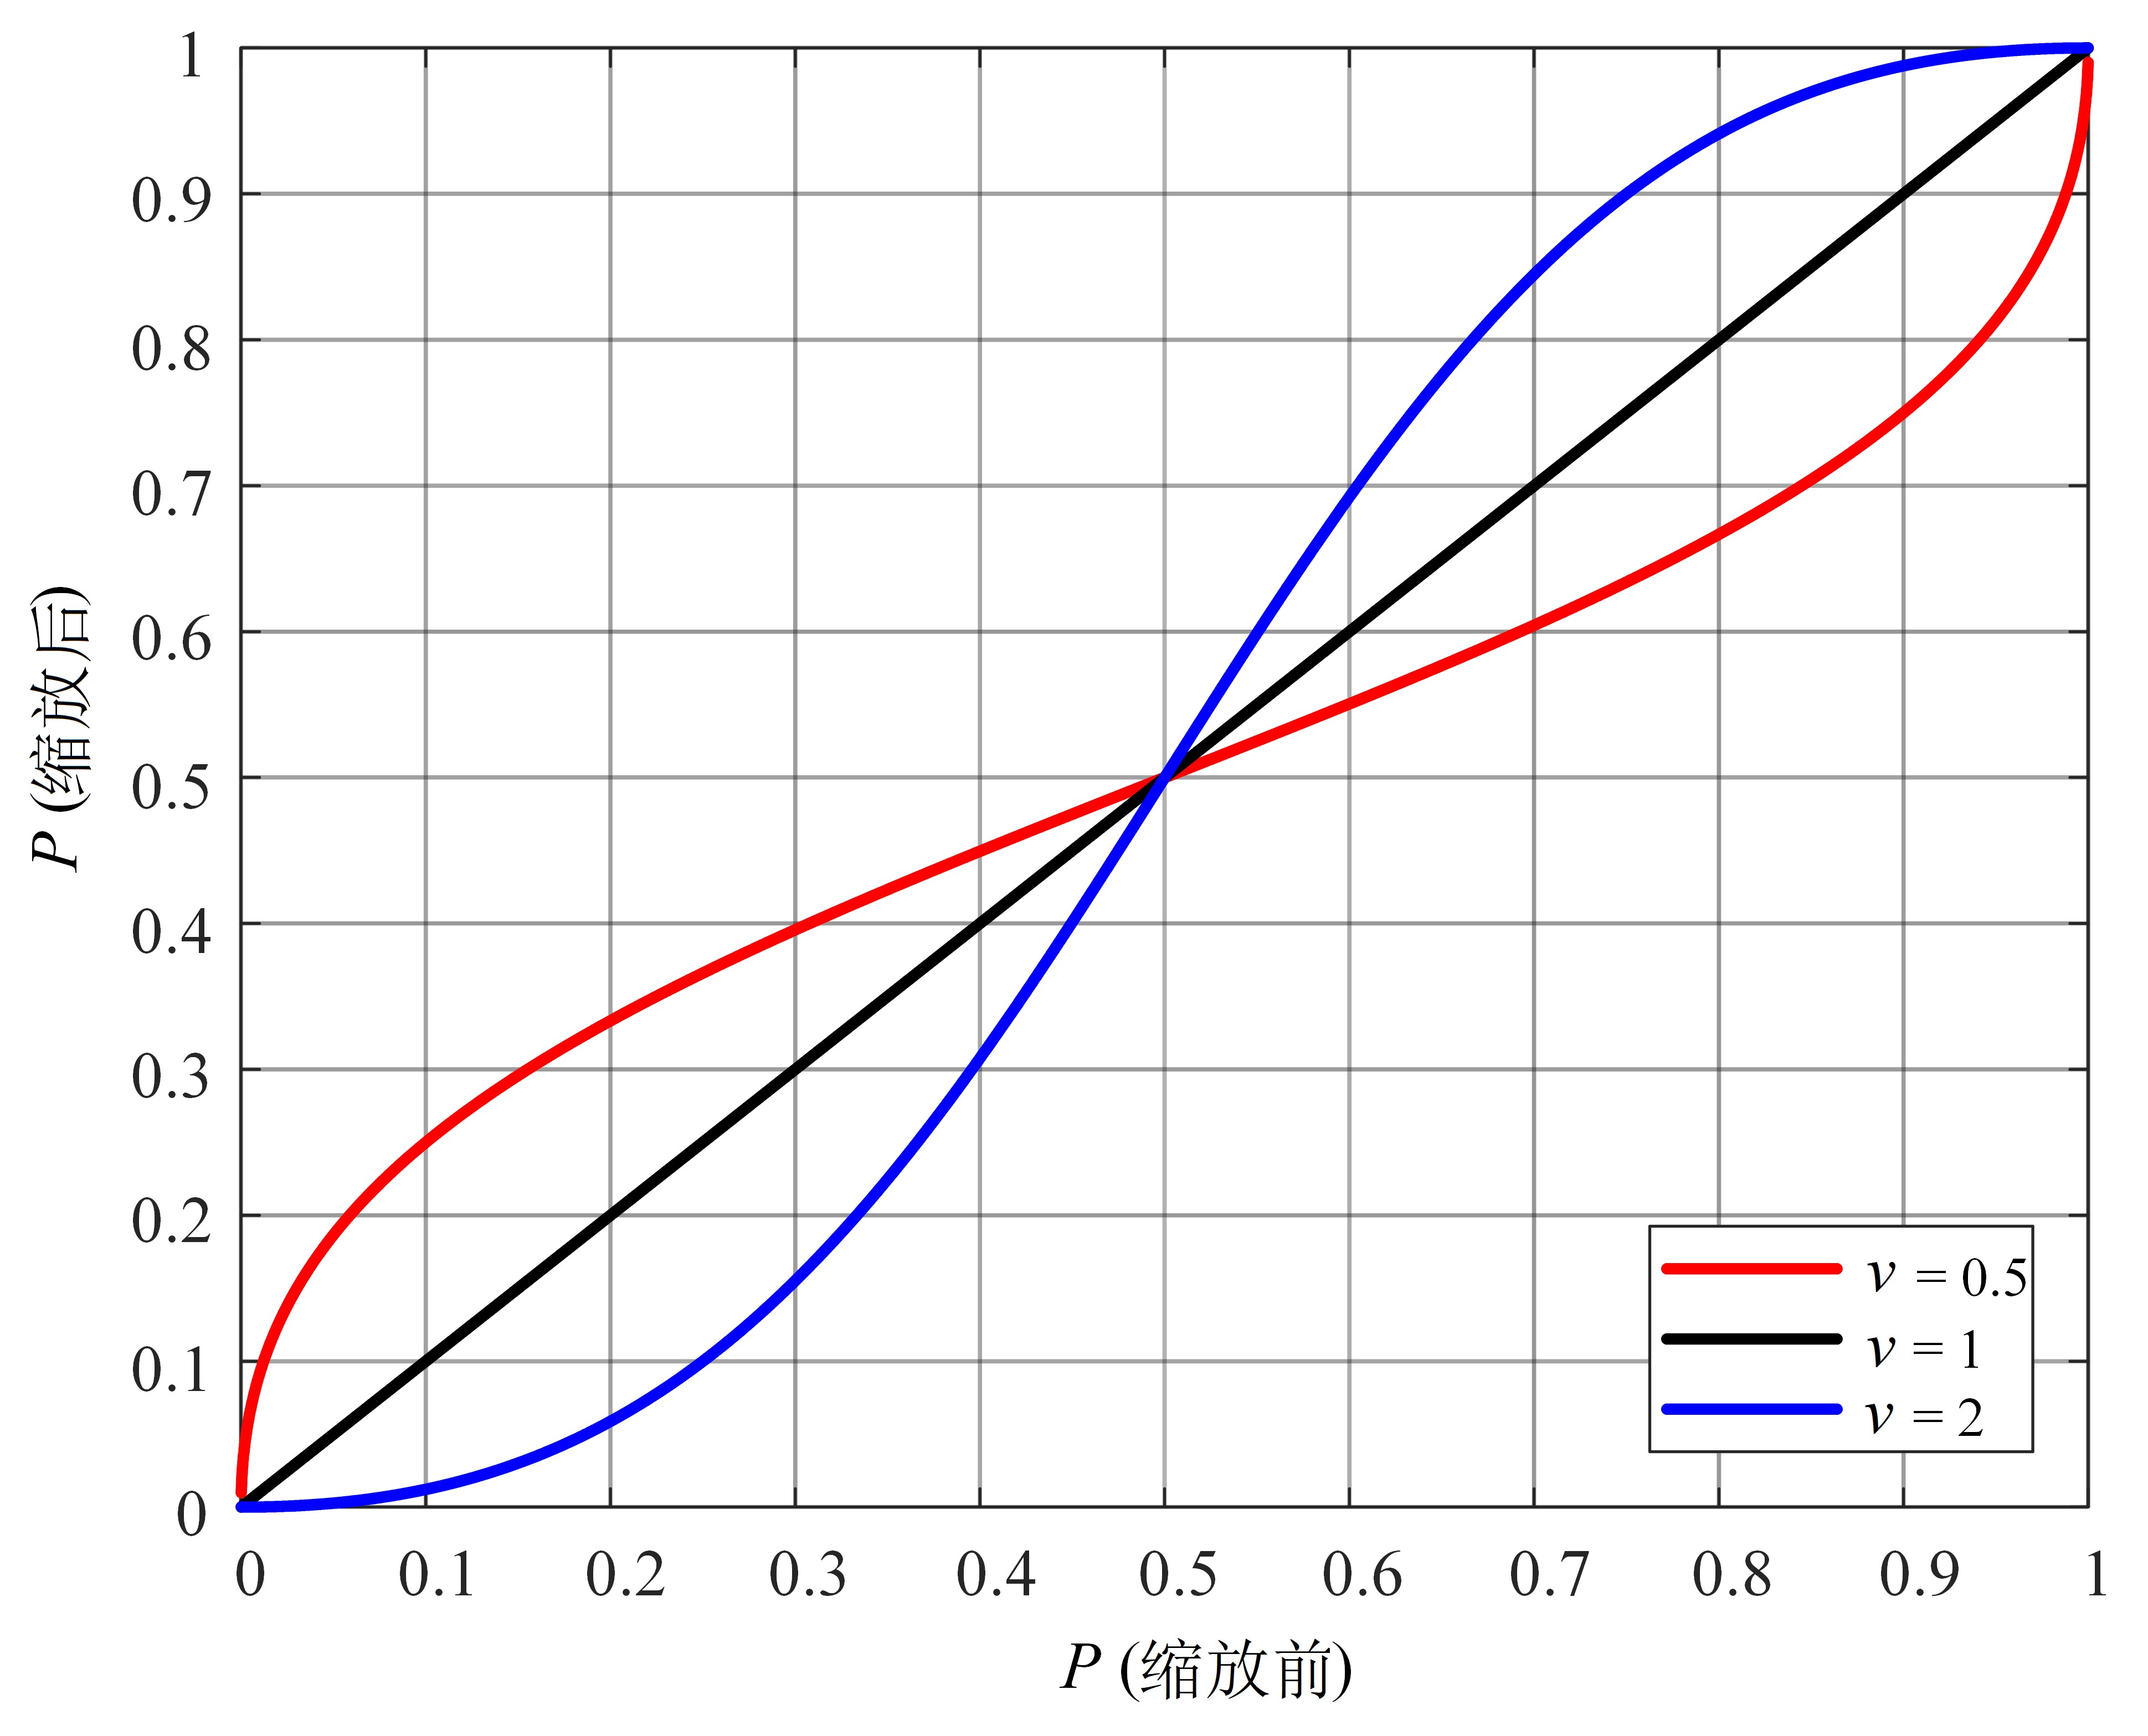
\includegraphics[width=10cm]{chapters/chapter3/31.jpg}
		\caption{\wuhao 不同缩放系数v的缩放结果} 
		\label{fig:3.1} 
		\wuhao Fig.3-1 Scaling results with different scaling coefficients ν
\end{figure}

%调整图片与下方文字之间的间距
\vspace{-0.5cm}

图片与上下文的间距由于LATEX动态排版特性,需要大家手动调整。
。

。

。

。

。

。

。

下图是多子图示例:
\vspace{-1cm}

\begin{figure}[h]
	\centering
	\subfigure[]{
		\label{fig:DE_J}
		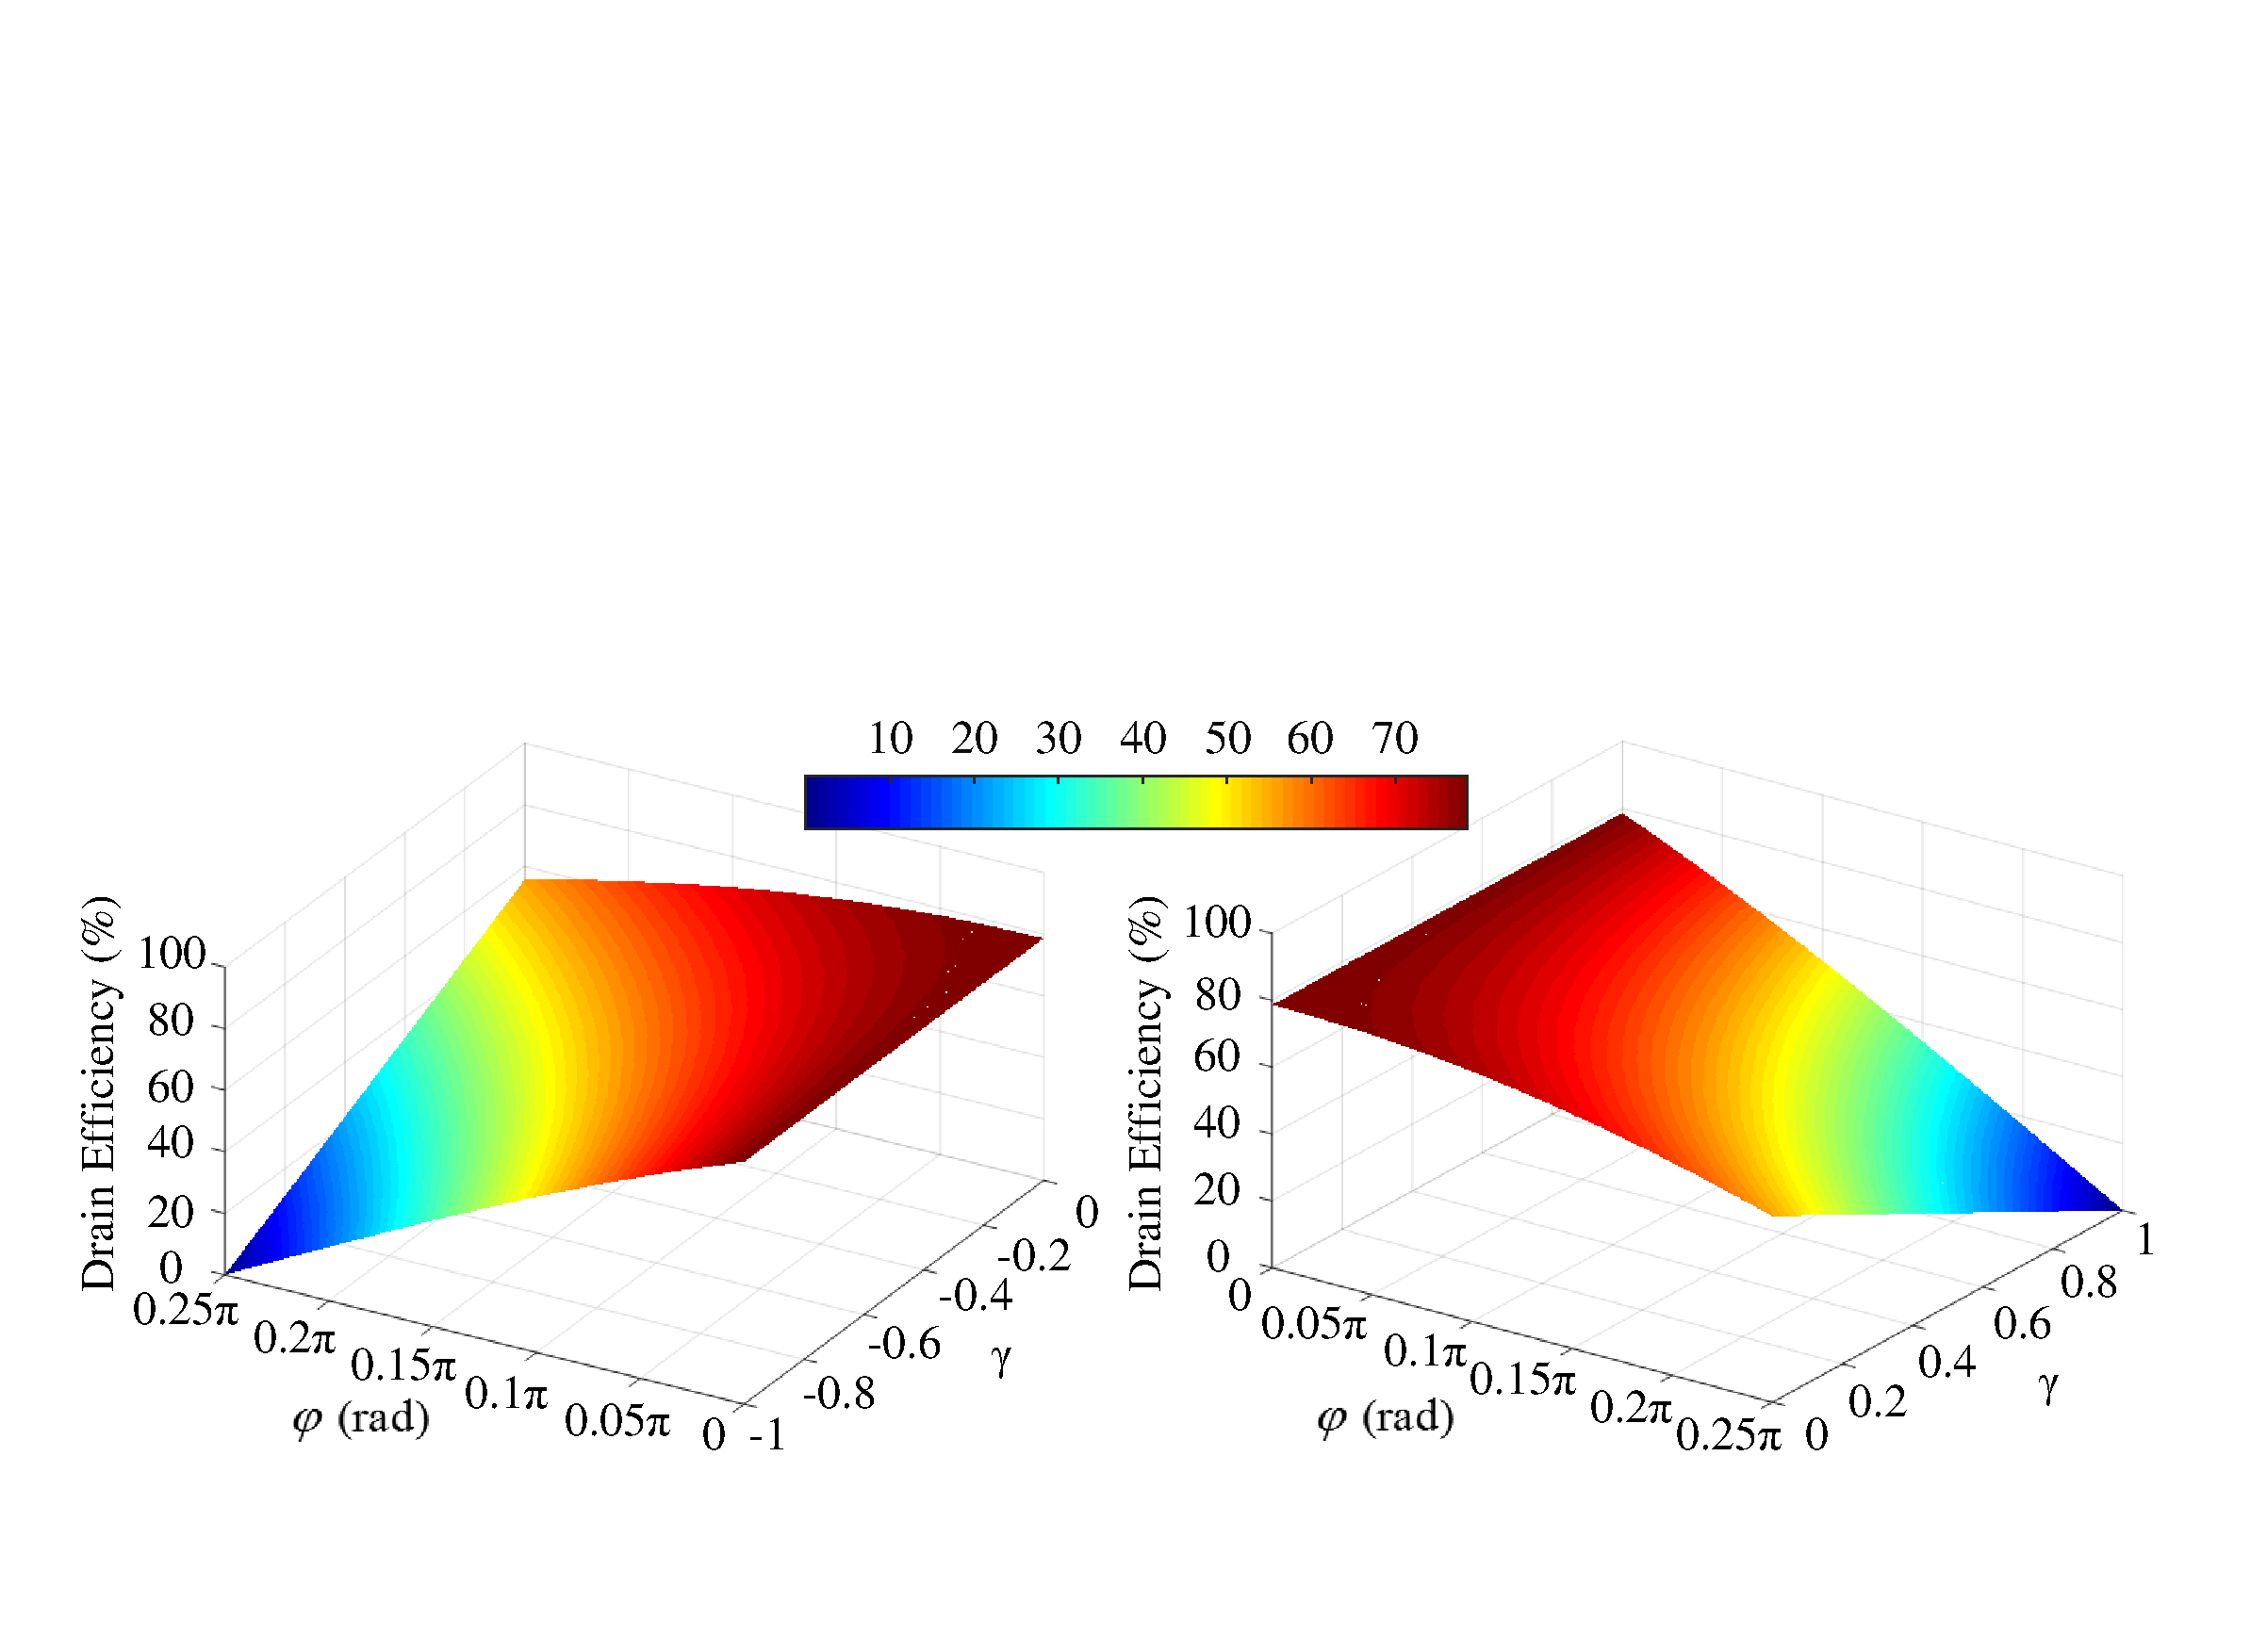
\includegraphics[width=12cm]{chapters/chapter3/DE_J.pdf}}
	\subfigure[]{
		\label{fig:DE_CF}
		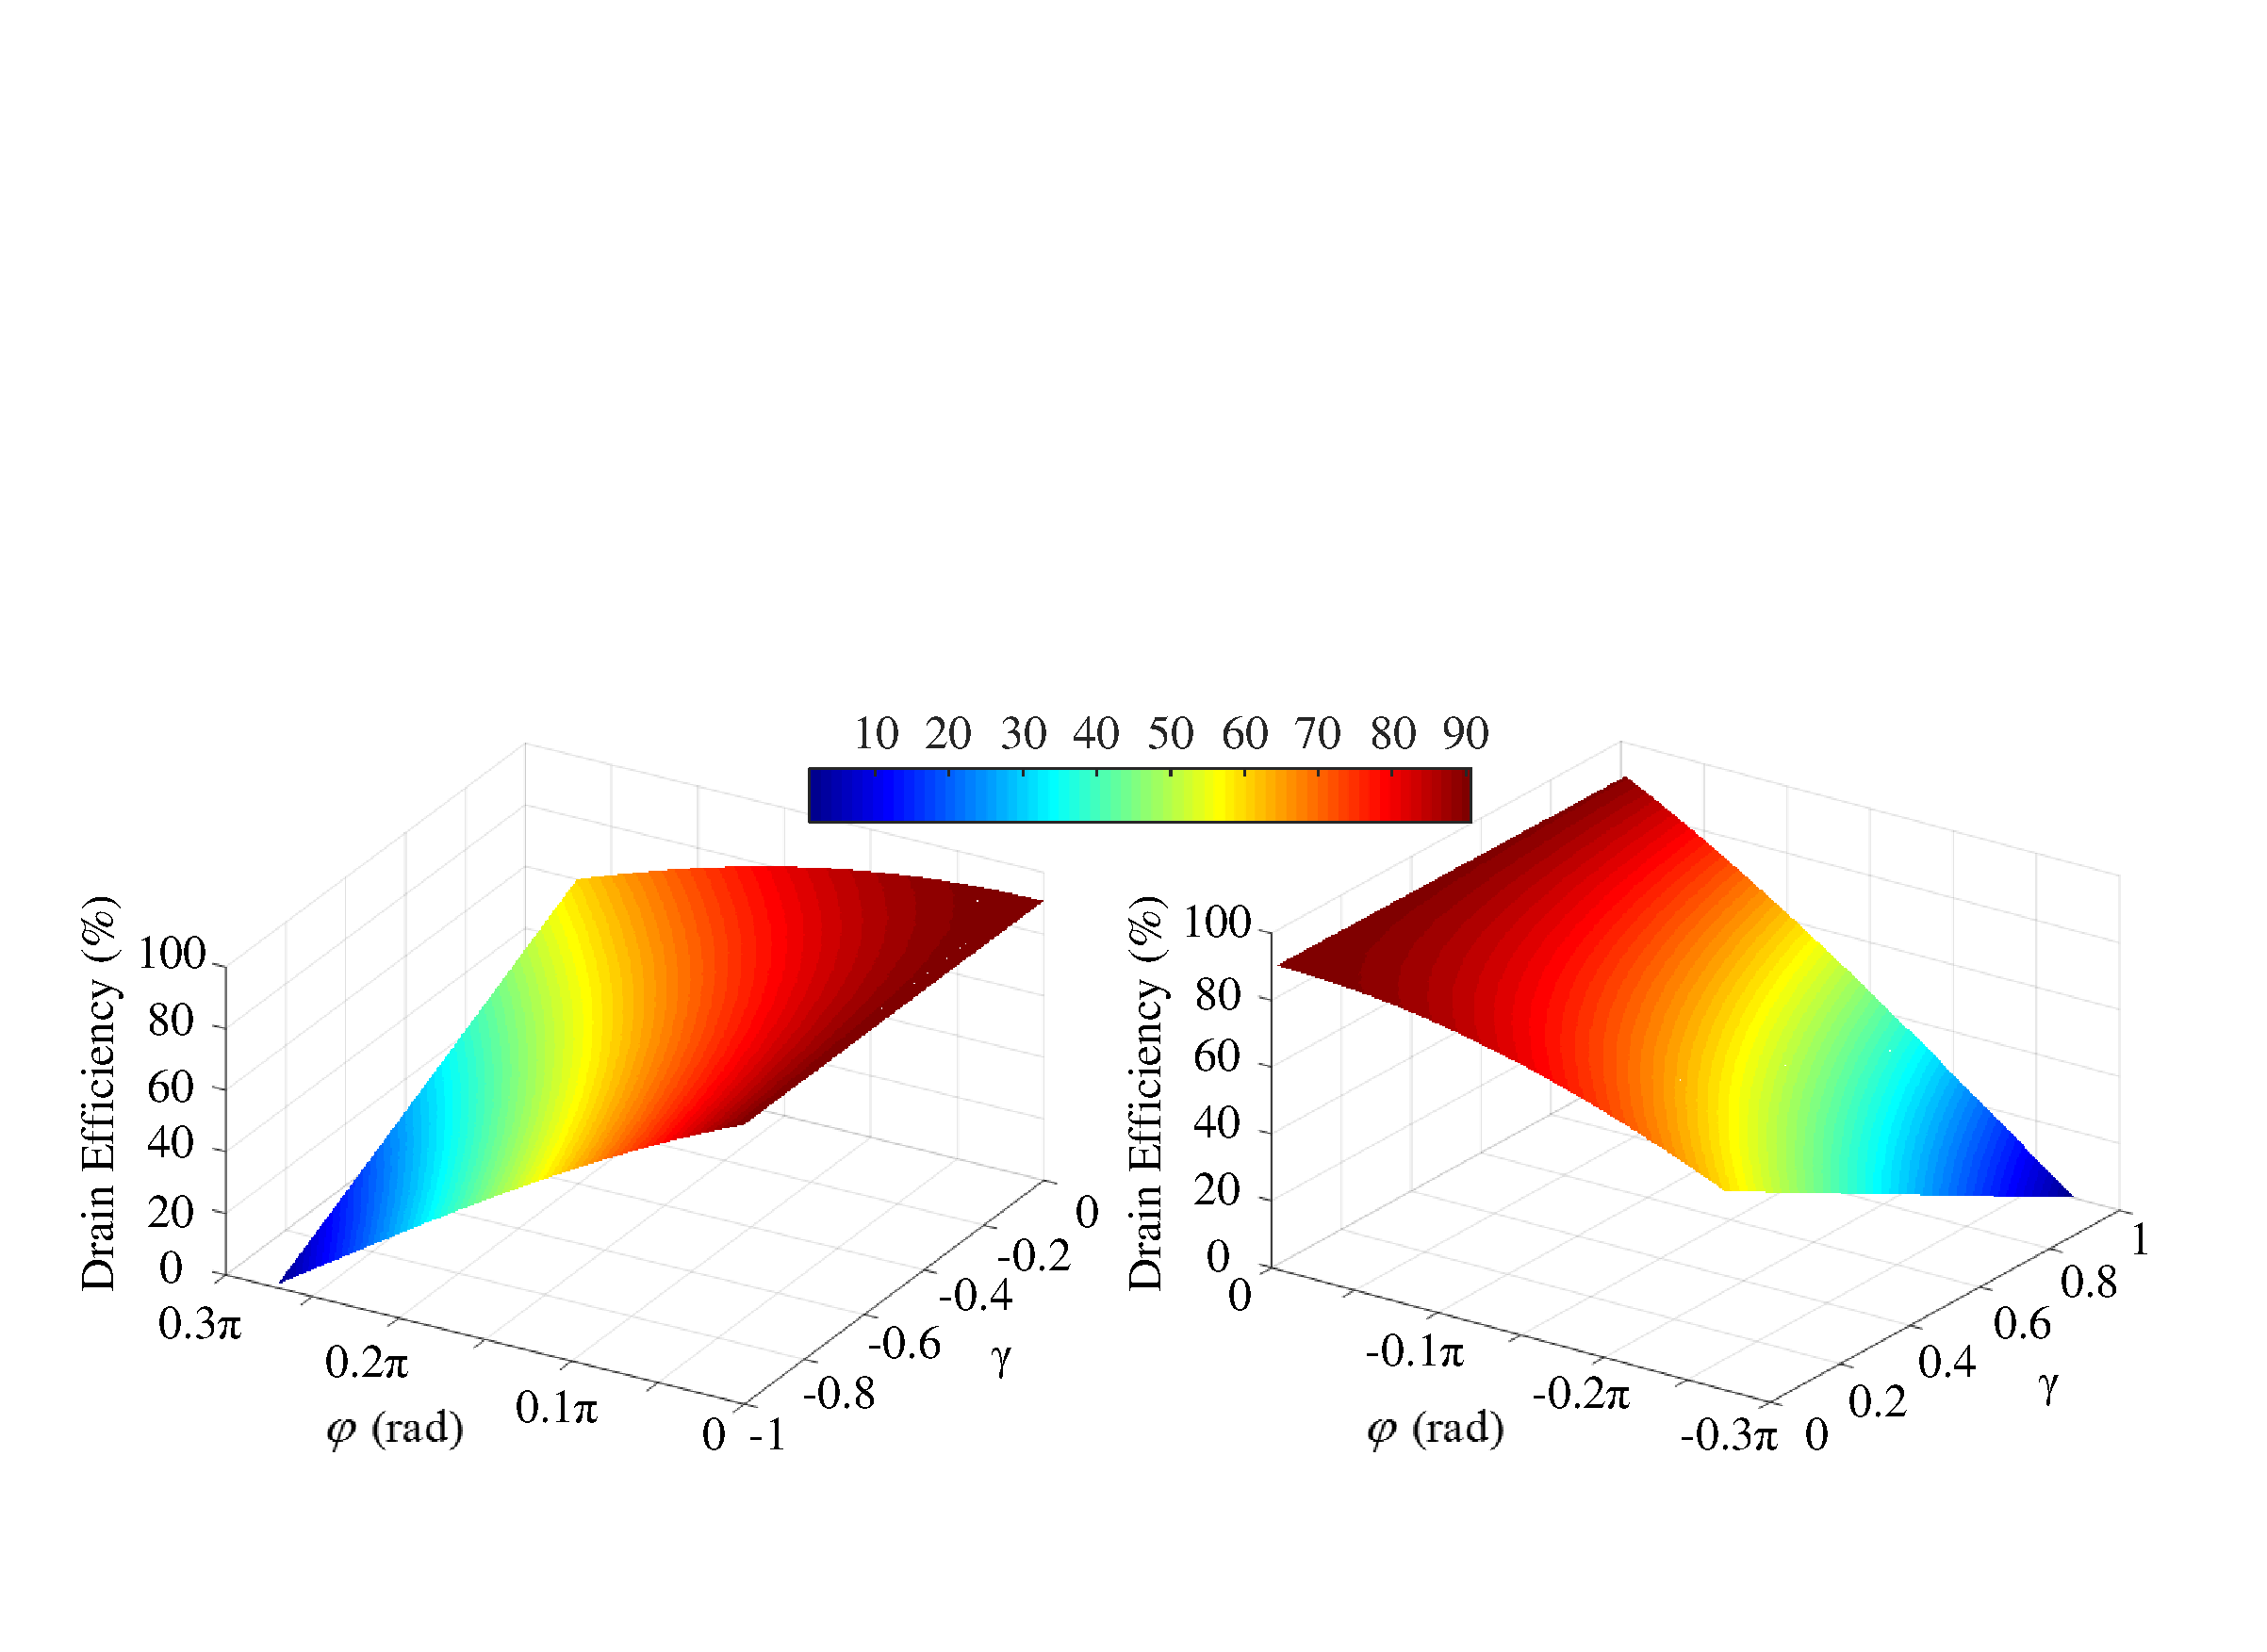
\includegraphics[width=12cm]{chapters/chapter3/DE_CF.pdf}}
	\caption{\wuhao 理论效率与$\gamma$和$\varphi$的关系. (a) $\alpha=1$. (b) $\alpha=2/\sqrt{3}$.}
	\wuhao Fig. 3-2 Theoretical DE versus $\gamma$ and $\varphi$. (a) $\alpha=1$. (b) $\alpha=2/\sqrt{3}$.
\end{figure}

\vspace{-0.5cm}

\subsubsection{表}

\begin{table}[h]
	\renewcommand{\arraystretch}{1.5}
	\centering
	\caption{\wuhao 电流类型对效率的影响}
	\wuhao Table3-1 Current type impact on efficiency
	\begin{tabular}{p{3cm}p{3cm}p{3cm}p{3cm}}
		\toprule[1.5pt]
		\makecell[c]{\songti\wuhao 电流类型}&\makecell[c]{\songti\wuhao A}&\makecell[c]{\songti\wuhao B}&\makecell[c]{\songti\wuhao C}\\
		\hline
		\makecell[c]{\wuhao aaa}&\makecell[c]{\wuhao aa1}&\makecell[c]{\wuhao bb1}&\makecell[c]{\wuhao cc1}\\
		\bottomrule[1.5pt]
	\end{tabular}
   \label{tab:3.1} 
	
\end{table}

\begin{table*}[tp]
	\renewcommand{\arraystretch}{1.5}
	\caption{\wuhao 高效率功放性能对比}
	\wuhao Table3-2 High-effiency power amplifier performance comparison 
	\label{tab_1}
	\centering
	\begin{tabular}{c c c c c }
		\hline
		{\textbf{带宽}(GHz)}&{\textbf{功率}(dBm)}&{\textbf{效率}(\%)}&{\textbf{线性度}(dBc)}&{\textbf{信号带宽}(MHz)}\\
		\hline
		1.4--2.6&32--34&30--40 (DE)&-25 -- -30 (ACLR)&5\\
		\hline
		\multirow{2}{*}{2.1--2.7}&39&45 (DE) @ 2.14 GHz&--31 (ACLR)&\multirow{2}{*}{5}\\\cline{3-4}
		&(average)&40 (DE) @ 2.655 GHz&--30 (ACLR)&\\
		\hline
		3.5&38.1&59 (PAE)&30 (C/I)&5\\
		\hline
		\multirow{2}{*}{1.6--2.6}&36.0--38.5&45--60 (PAE)&30 (C/I)&5\\\cline{2-5}
		&35.3--37.5&40--55 (PAE)&--30 (ACLR)&20\\
		\hline
	\end{tabular}
\end{table*}


\subsection{公式格式}

\begin{equation}
\left\{ \begin{aligned}
0.794 \le \zeta  \le 1 ~~~~~~~~~~~\\
0.631 \le \gamma  = \frac{{0.631}}{{{\zeta ^2}}} \le 1~~~~~~ \\
- \frac{1}{{2\gamma }} \le \delta  \le \frac{1}{{2\gamma }}~~~~~~~~~~~ \\
{Z_{c,low,f}} = 2{R_{opt}}(\gamma  + j\delta )~~~~~\\
{Z_{c,2f}} = {Z_{c,low,2f}} =  - j\frac{{3\pi }}{4}\gamma \delta {R_{opt}}
\end{aligned} \right.
\label{eq:3.1}
\end{equation}

\begin{equation}
\begin{aligned}
v(\theta ) = V_{DD}\cdot(1 - \alpha cos(\theta  + \varphi ) + \beta cos(3\theta  + 3\varphi ))\\
\cdot(1 - \gamma \sin (\theta  + \varphi )) ~~~~~- 1 \le \gamma  \le 1\
\end{aligned}
\label{eq:vd}
\end{equation}

\subsection{印制要求}
涉密学位论文的印刷、制作、传递、存档等,须符合国家、学校相关保密要求。学位论文一律左侧装订。

中文摘要之前的前置部分(封面、中、英文题名页、独创性声明和使用授权书),采用单面印刷。

从中文摘要开始,采用双面印刷。

中文摘要及之后的前置部分,包括中文摘要、ABSTRACT、目录、图目录(如有)、表目录(如有)、主要符号表(如有)、缩略词表(如有),在双面印刷时,若某部分页数为奇数,则该部分最后一页单面印刷。例如:若“摘要”只有1页,则其页码是“Ⅰ”,第“Ⅰ”页纸的背面为空白(无页眉或页码);“ABSTRACT”用新的一张纸印刷,页码从“Ⅱ”开始。

从第1章第1页开始,至论文最后1页,所有页面均双面印刷。例如:若第1章的最后1页为第17页,则第2章的第1页在第17页的背面印刷,页码为“18”(页眉是“重庆邮电大学博士(硕士)学位论文”)。

一次性双面打印整本学位论文技巧:除用于打印的版本外,电子版论文中一律不得出现空白页。论文打印建议使用PDF格式。为方便一次性双面打印,有时可在单面印刷的部分(如封面、中、英文题名页、独创性声明和使用授权书),或者双面打印只有1页的某部分内容(如摘要、ABSTRACT等)后插入1页空白页,该空白页不编排页眉页码;论文中出现的页码应前后连续,不得中断。

\subsection{算法流程}

\begin{algorithm}[htb]
	%	\renewcommand{\algorithmicrequire}{\textbf{Input:}}
	%	\renewcommand{\algorithmicensure}{\textbf{Output:}}
		\caption{xxx的算法流程}\label{algo1}
		\setlength{\baselineskip}{18bp}
		\begin{algorithmic}[1]
			\Require {原始图像: $ X $; 目标图像: $ Y $;;小批量数据采样器: $ SA $; 批次大小: $ k $; 学习率:$ lr $。}
			\Ensure {$F$,参数为$ \theta_1 $。}
			\State \textbf{初始化:} $ F $中的参数为 $\theta_1$ ; $ R $中的参数为$ \theta_2 $;$ D $中的参数为$ \theta_3 $。
			\While {$ \theta_1 $未收敛}
			\State $ \left(x,y\right)\gets SA\left(X,Y\right) $ \{采样批次大小为$k$的图像\};
			\State  $ y^{\prime}\gets F_{\theta_1}\left(x\right) $ \{利用源图像前向合成目标图像 \};
			\State $ {y^\prime}_r\gets{y\prime\circ R}_{\theta_2}\left(y^\prime,y\right) $ \{使用合成的图像$y^{\prime}$ 和真实图像 $ y $前向配准 \};
			\State $ {y_{em}^{\prime}\gets D}_{\theta_3}\left(y^\prime\right) $ \{获取合成图像的特征嵌入\};
			\State $ {y_{em}\gets D}_{\theta_3}\left(y\right) $ \{获取真实图像的特征嵌入\};
			\State 利用公式\ref{eq:3.1}计算关于参数$\theta_2$的梯度;
			\State 利用公式\ref{eq:3.1}计算关于参数$\theta_1$的梯度;
			\State $ \theta_2\gets\theta_2-lr \cdot\frac{\partial L_{total}}{\partial\theta_2}\ $ \{更新分布校正器$ R $的参数$\theta_2$ \};
			\State $ \theta_1\gets\theta_1-lr\cdot\frac{\partial L_{total}}{\partial\theta_1} $ \{更新分布生成器 $ F $的参数$\theta_1$ \};
			\State $ y_a\gets D_{\theta_3}\left(y\right) $ \{构建锚点样本 \};
			\State 随机打乱锚点样本,构造正样本$ y_p $;
			\State 随机打乱$ D_{\theta_3}(y^{\prime}) $,构造负样本$ y_n $;
			\State 利用公式\ref{eq:3.1}计算关于参数$ \theta_3 $的梯度;
			\State $ \theta_3\gets\theta_3-lr\cdot\frac{\partial L_{total}}{\partial\theta_3} $ \{更新分布鉴别器$ D $的参数$\theta_3$ \};
			\EndWhile
		\end{algorithmic}
	\end{algorithm}

\subsection{本章小结}
本章介绍了……